\documentclass[a4paper, 13pt, onesided]{article} % for A4 size paper
\usepackage{tikz}
\usepackage{pdfpages}


\newcommand\nrOfPages{8}

% Blank pages
\newcommand{\insertPage}[0]{
	\newpage
	\begin{tikzpicture}[remember picture, overlay]
	
	\tikzset{normal lines/.style={gray, very thin}} 
	\tikzset{margin lines/.style={gray, thick}} 
	\tikzset{mm lines/.style={gray, ultra thin}} 
	\tikzset{strong lines/.style={black, very thin}} 
	\tikzset{master lines/.style={black, very thick}} 
	\tikzset{dashed master lines/.style={loosely dashed, black, very thick}} 
	
	\node at (current page.south west){
		\begin{tikzpicture}[remember picture, overlay]
		
		\draw[style=normal lines,step=0.3cm] (0,0) grid +(210mm,297mm); 
		
		\end{tikzpicture}
	};
	\end{tikzpicture}
}


%%%%%%%%%%%%%%%%%%%
% DOCUMENT
\begin{document}
	
\pagenumbering{gobble} % Disable page numbering
%%%%%%%%%%%%%%%%%%%
% Titlepage
\title{Summary for Analysis of Sequential Data,\\TSM\_AnSeqDa}
\date{\today}
% TODO: Place your name here!
\author{J.~R.~R.~Tolkien\\HS 2018/19}
\maketitle
\clearpage


%%%%%%%%%%%%%%%%%%%
% Insert blank pages
\makeatletter
\newcounter{int}
\@whilenum\value{int}<\nrOfPages\do
{\stepcounter{int}\insertPage}
\makeatother


%%%%%%%%%%%%%%%%%%%
% Normal Distribution Table
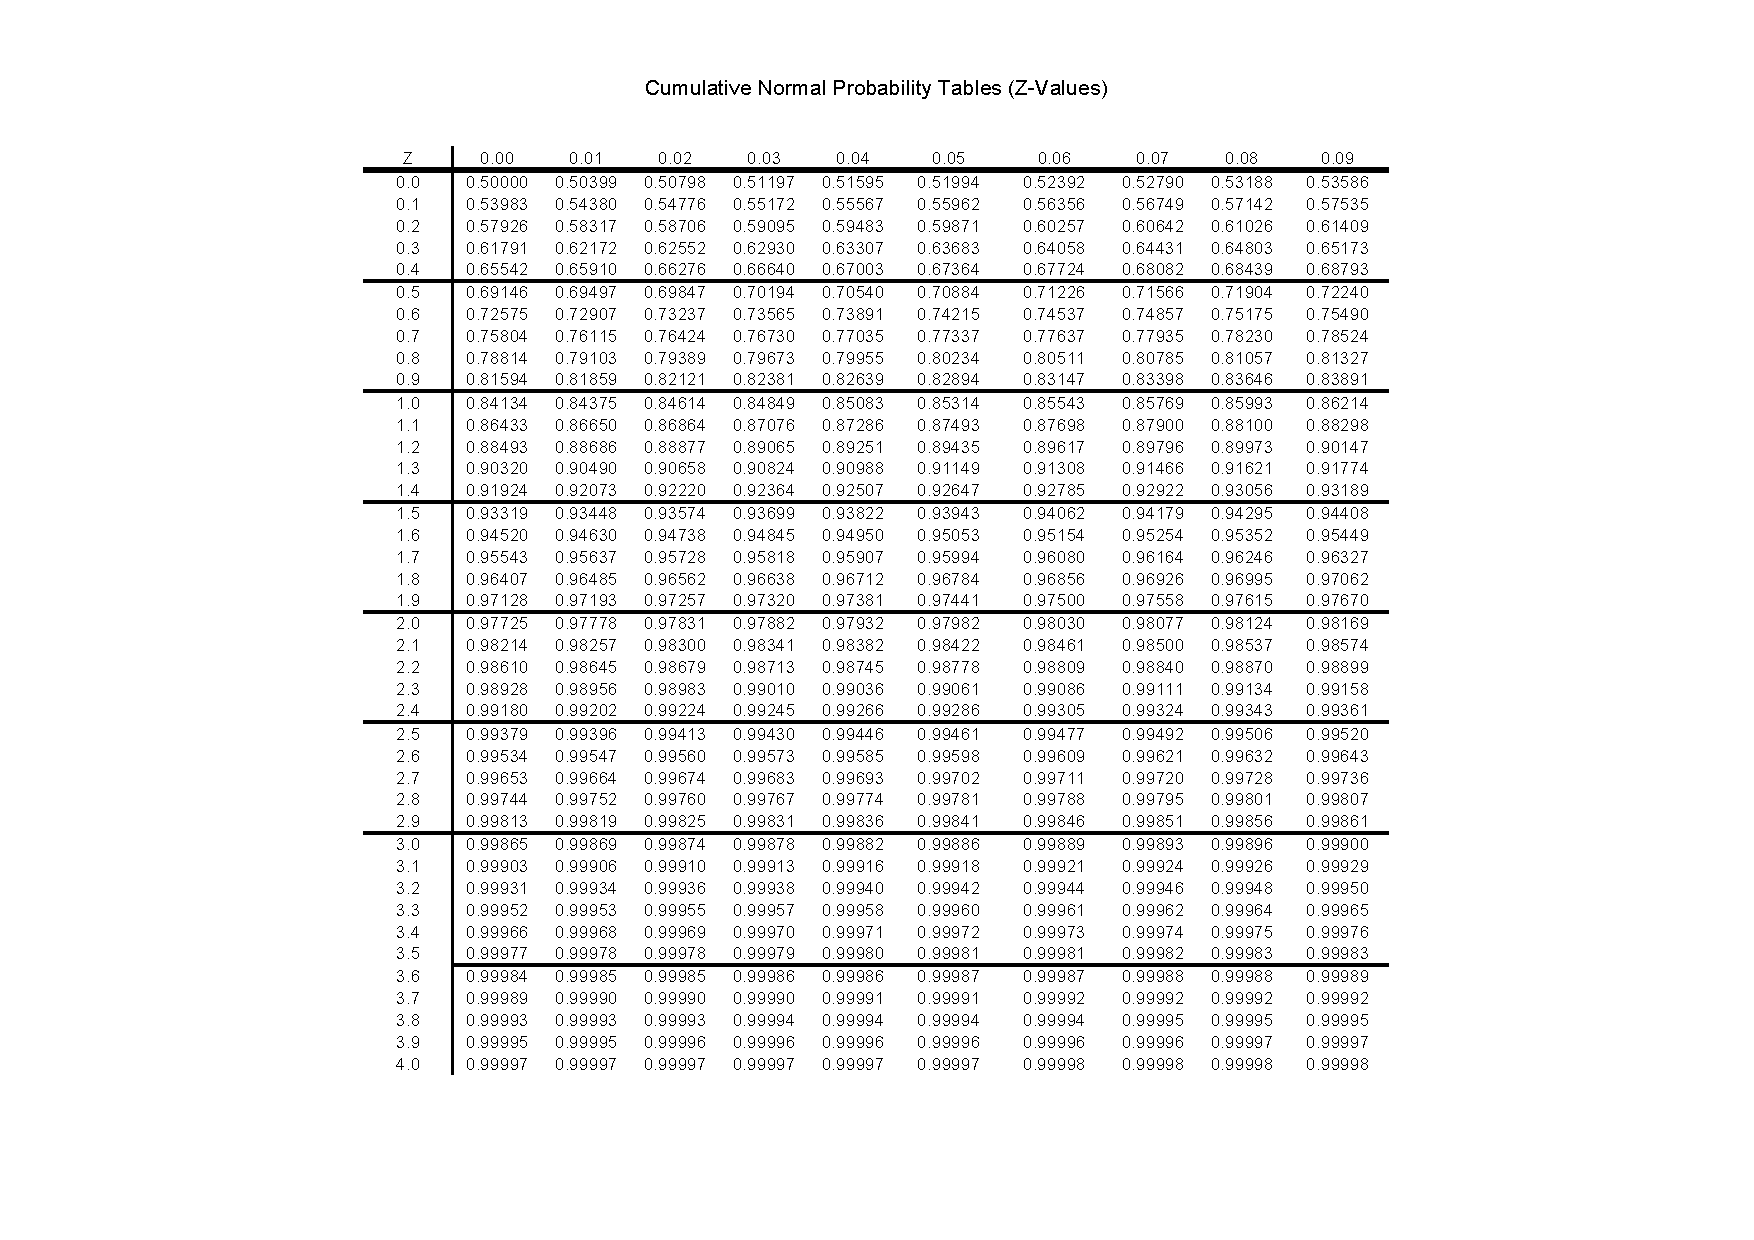
\includepdf[pages=-, angle=90]{normal-standard}

\end{document}
